\documentclass{article}
\usepackage[dvipsnames,svgnames,x11names]{xcolor}
\usepackage{tikz}
\usepackage{amsmath}
\usepackage{amssymb}
\usepackage{geometry}
\usepackage{subcaption}
\pagecolor{white}

\usetikzlibrary{backgrounds}
\usetikzlibrary{arrows.meta}
\usetikzlibrary{fit}

% Multiplication table styles
\tikzstyle{cell} = [rectangle, minimum size=2cm, draw=black, thick, align=center]
\tikzstyle{headcell} = [rectangle, minimum size=2cm, draw=black, line width=2.5, align=center]

\colorlet{red}{Firebrick1}
\colorlet{orange}{orange}
\colorlet{yellow}{yellow}
\colorlet{green}{LimeGreen}
\colorlet{blue}{ProcessBlue}
\colorlet{purple}{BlueViolet}

\colorlet{dred}{Firebrick3}
\colorlet{dorange}{orange}
\colorlet{dyellow}{Gold2}
\colorlet{dgreen}{Green4}
\colorlet{dblue}{DodgerBlue4}
\colorlet{dpurple}{BlueViolet}

\tikzstyle{symbolcell} = [headcell, fill=white]
\tikzstyle{headtau} = [headcell, fill=gray!70]
\tikzstyle{headi1} = [headcell, fill=red!70]
\tikzstyle{heade1} = [headcell, fill=orange!70]
\tikzstyle{headi2} = [headcell, fill=yellow!70]
\tikzstyle{heade2} = [headcell, fill=green!70]
\tikzstyle{headi3} = [headcell, fill=blue!70]
\tikzstyle{heade3} = [headcell, fill=purple!70]

\tikzstyle{zerocell} = [cell, fill=white]
\tikzstyle{taucell} = [cell, fill=gray!60]
\tikzstyle{i1cell} = [cell, fill=red!60]
\tikzstyle{e1cell} = [cell, fill=orange!60]
\tikzstyle{i2cell} = [cell, fill=yellow!60]
\tikzstyle{e2cell} = [cell, fill=green!60]
\tikzstyle{i3cell} = [cell, fill=blue!60]
\tikzstyle{e3cell} = [cell, fill=purple!60]

\def \1e{\tau}
\def\2e{x}
\def\3e{t_x}
\def\4e{y}
\def\5e{t_y}
\def\6e{z}
\def\7e{t_z}


    
\begin{document}





\begin{figure}[htbp]
\newsavebox{\lefttableboxA}
\newsavebox{\righttableboxA}
\sbox{\lefttableboxA}{
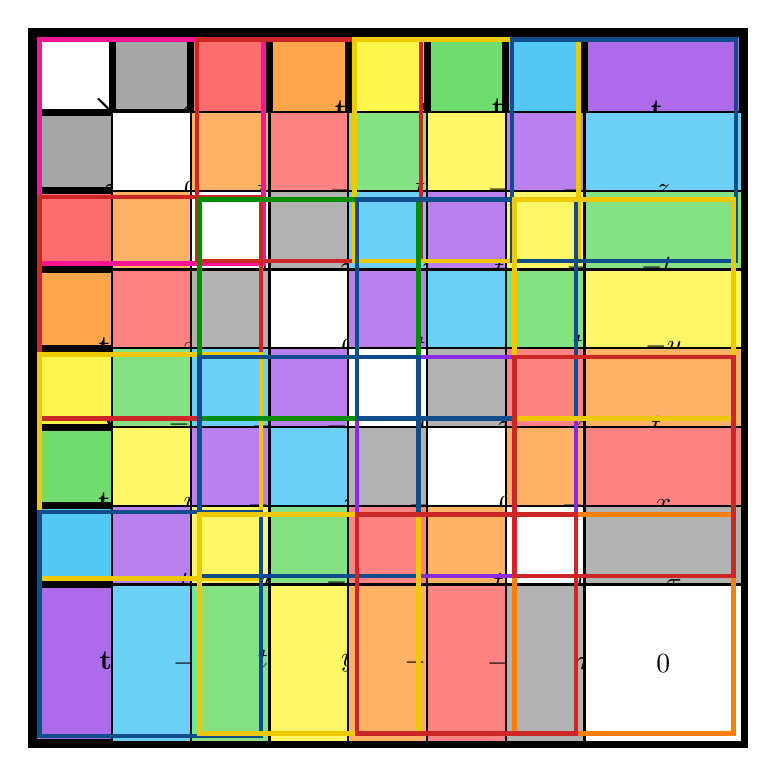
\begin{tikzpicture}[baseline=(current bounding box.north)]

% i in {x, y, z} thus t_i in {t_x, t_y, t_z}
% and (i, t_i) in {(x, t_x), (y, t_y), (z, t_z)}.
% Multiplication table row and column labels:
% Table product symbol
\node[symbolcell] (n00) at (0, 0) {{\huge $\mathbf{\times}$}};
% Column headers, {e_U: (tau, (i, t_i)) }
\node[headtau] (n01) at (1, 0) {$\mathbf{\tau}$};
\node[headi1] (n02) at (2, 0) {$\mathbf{x}$};
\node[heade1] (n03) at (3, 0) {$\mathbf{t_x}$};
\node[headi2] (n04) at (4, 0) {$\mathbf{y}$};
\node[heade2] (n05) at (5, 0) {$\mathbf{t_y}$};
\node[headi3] (n06) at (6, 0) {$\mathbf{z}$};
\node[heade3] (n07) at (7, 0) {$\mathbf{t_z}$};
% Row headers, {e_U: (tau, (i, t_i)) }
\node[headtau] (n10) at (0, -1) {$\mathbf{\tau}$};
\node[headi1] (n20) at (0, -2) {$\mathbf{x}$};
\node[heade1] (n30) at (0, -3) {$\mathbf{t_x}$};
\node[headi2] (n40) at (0, -4) {$\mathbf{y}$};
\node[heade2] (n50) at (0, -5) {$\mathbf{t_y}$};
\node[headi3] (n60) at (0, -6) {$\mathbf{z}$};
\node[heade3] (n70) at (0, -7) {$\mathbf{t_z}$};
% Multiplication table cells:
% Row 1, {tau: (tau, (i, t_i)) }
\node[zerocell] (n11) at (1, -1) {$0$};
\node[e1cell] (n12) at (2, -1) {$t_x$};
\node[i1cell] (n13) at (3, -1) {$-x$};
\node[e2cell] (n14) at (4, -1) {$t_y$};
\node[i2cell] (n15) at (5, -1) {$-y$};
\node[e3cell] (n16) at (6, -1) {$-t_z$};
\node[i3cell] (n17) at (7, -1) {$z$};
% Row 2, {x: (tau, (i, t_i)) }
\node[e1cell] (n21) at (1, -2) {$-t_x$};
\node[zerocell] (n22) at (2, -2) {$0$};
\node[taucell] (n23) at (3, -2) {$\tau$};
\node[i3cell] (n24) at (4, -2) {$z$};
\node[e3cell] (n25) at (5, -2) {$t_z$};
\node[i2cell] (n26) at (6, -2) {$-y$};
\node[e2cell] (n27) at (7, -2) {$-t_y$};
% Row 3, {t_x: (tau, (i, t_i)) }
\node[i1cell] (n31) at (1, -3) {$x$};
\node[taucell] (n32) at (2, -3) {$-\tau$};
\node[zerocell] (n33) at (3, -3) {$0$};
\node[e3cell] (n34) at (4, -3) {$t_z$};
\node[i3cell] (n35) at (5, -3) {$-z$};
\node[e2cell] (n36) at (6, -3) {$t_y$};
\node[i2cell] (n37) at (7, -3) {$-y$};
% Row 4, {y: (tau, (i, t_i)) }
\node[e2cell] (n41) at (1, -4) {$-t_y$};
\node[i3cell] (n42) at (2, -4) {$-z$};
\node[e3cell] (n43) at (3, -4) {$-t_z$};
\node[zerocell] (n44) at (4, -4) {$0$};
\node[taucell] (n45) at (5, -4) {$\tau$};
\node[i1cell] (n46) at (6, -4) {$x$};
\node[e1cell] (n47) at (7, -4) {$t_x$};
% Row 5, {t_y: (tau, (i, t_i)) }
\node[i2cell] (n51) at (1, -5) {$y$};
\node[e3cell] (n52) at (2, -5) {$-t_z$};
\node[i3cell] (n53) at (3, -5) {$z$};
\node[taucell] (n54) at (4, -5) {$-\tau$};
\node[zerocell] (n55) at (5, -5) {$0$};
\node[e1cell] (n56) at (6, -5) {$-t_x$};
\node[i1cell] (n57) at (7, -5) {$x$};
% Row 6, {z: (tau, (i, t_i)) }
\node[e3cell] (n61) at (1, -6) {$t_z$};
\node[i2cell] (n62) at (2, -6) {$y$};
\node[e2cell] (n63) at (3, -6) {$-t_y$};
\node[i1cell] (n64) at (4, -6) {$-x$};
\node[e1cell] (n65) at (5, -6) {$t_x$};
\node[zerocell] (n66) at (6, -6) {$0$};
\node[taucell] (n67) at (7, -6) {$-\tau$};
% Row 7, {t_z: (tau, (i, t_i)) }
\node[i3cell] (n71) at (1, -7) {$-z$};
\node[e2cell] (n72) at (2, -7) {$t_y$};
\node[i2cell] (n73) at (3, -7) {$y$};
\node[e1cell] (n74) at (4, -7) {$-t_x$};
\node[i1cell] (n75) at (5, -7) {$-x$};
\node[taucell] (n76) at (6, -7) {$\tau$};
\node[zerocell] (n77) at (7, -7) {$0$};
% BOXING
% frame
\node[draw, ultra thick, black, fit=(n00) (n70) (n07) (n77), inner sep=0pt] {};
% headings, and tau (universal turn mixing)
\node[draw, ultra thick, DeepPink1, fit=(n00) (n01) (n10) (n11), inner sep=-3.5pt] {};
\node[draw, ultra thick, dred, fit=(n02) (n03) (n12) (n13), inner sep=-3.5pt] {};
\node[draw, ultra thick, dyellow, fit=(n04) (n05) (n14) (n15), inner sep=-3.5pt] {};
\node[draw, ultra thick, dblue, fit=(n06) (n07) (n16) (n17), inner sep=-3.5pt] {};
\node[draw, ultra thick, dred, fit=(n20) (n21) (n21) (n31), inner sep=-3.5pt] {};
\node[draw, ultra thick, dyellow, fit=(n40) (n50) (n41) (n51), inner sep=-3.5pt] {};
\node[draw, ultra thick, dblue, fit=(n60) (n70) (n61) (n71), inner sep=-3.5pt] {};
% diagonals (intrasector mixing)
\node[draw, ultra thick, dgreen, fit=(n22) (n23) (n32) (n33), inner sep=-3.5pt] {};
\node[draw, ultra thick, dpurple, fit=(n44) (n45) (n54) (n55), inner sep=-3.5pt] {};
\node[draw, ultra thick, dorange, fit=(n66) (n67) (n76) (n77), inner sep=-3.5pt] {};
% ie pair blocks (intersector mixing)
\node[draw, ultra thick, dblue, fit=(n24) (n25) (n34) (n35), inner sep=-3.5pt] {};
\node[draw, ultra thick, dyellow, fit=(n26) (n27) (n36) (n37), inner sep=-3.5pt] {};
\node[draw, ultra thick, dred, fit=(n46) (n47) (n56) (n57), inner sep=-3.5pt] {};
\node[draw, ultra thick, dblue, fit=(n42) (n52) (n43) (n53), inner sep=-3.5pt] {};
\node[draw, ultra thick, dyellow, fit=(n62) (n72) (n63) (n73), inner sep=-3.5pt] {};
\node[draw, ultra thick, dred, fit=(n64) (n74) (n65) (n75), inner sep=-3.5pt] {};
\end{tikzpicture} }

\sbox{\righttableboxA}{
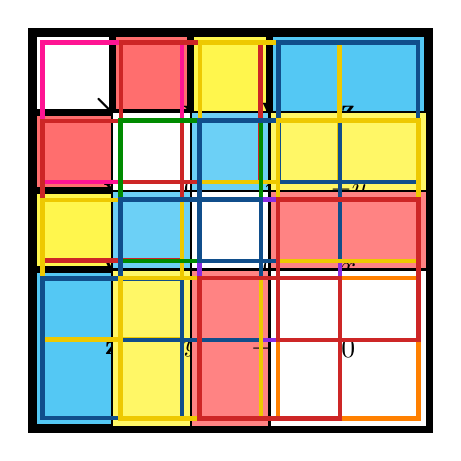
\begin{tikzpicture}
% i in {x, y, z}.
% Multiplication table row and column labels:
% Table product symbol
\node[symbolcell] (n00) at (0, 0) {{\huge $\mathbf{\times}$}};
% Column headers, {e_i: (i) }
\node[headi1] (n01) at (1, 0) {$\mathbf{x}$};
\node[headi2] (n02) at (2, 0) {$\mathbf{y}$};
\node[headi3] (n03) at (3, 0) {$\mathbf{z}$};
% Row headers {e_i: (i) }
\node[headi1] (n10) at (0, -1) {$\mathbf{x}$};
\node[headi2] (n20) at (0, -2) {$\mathbf{y}$};
\node[headi3] (n30) at (0, -3) {$\mathbf{z}$};
% Multiplication table cells:
% Row 1, {x: (i) }
\node[zerocell] (n11) at (1, -1) {$0$};
\node[i3cell] (n12) at (2, -1) {$z$};
\node[i2cell] (n13) at (3, -1) {$-y$};
% Row 2, {y: (i) }
\node[i3cell] (n21) at (1, -2) {$-z$};
\node[zerocell] (n22) at (2, -2) {$0$};
\node[i1cell] (n23) at (3, -2) {$x$};
% Row 3, {z: (i) }
\node[i2cell] (n31) at (1, -3) {$y$};
\node[i1cell] (n32) at (2, -3) {$-x$};
\node[zerocell] (n33) at (3, -3) {$0$};
% BOXING
% frame
\node[draw, ultra thick, black, fit=(n00) (n30) (n03) (n33), inner sep=0pt] {};
% headings, and tau (universal turn mixing)
\node[draw, ultra thick, DeepPink1, fit=(n00), inner sep=-4.5pt] {};
\node[draw, ultra thick, dred, fit=(n01), inner sep=-4.5pt] {};
\node[draw, ultra thick, dyellow, fit=(n02), inner sep=-4.5pt] {};
\node[draw, ultra thick, dblue, fit=(n03), inner sep=-4.5pt] {};
\node[draw, ultra thick, dred, fit=(n10), inner sep=-4.5pt] {};
\node[draw, ultra thick, dyellow, fit=(n20), inner sep=-4.5pt] {};
\node[draw, ultra thick, dblue, fit=(n30), inner sep=-4.5pt] {};
% diagonals (intrasector mixing)
\node[draw, ultra thick, dgreen, fit=(n11), inner sep=-3.5pt] {};
\node[draw, ultra thick, dpurple, fit=(n22), inner sep=-3.5pt] {};
\node[draw, ultra thick, dorange, fit=(n33), inner sep=-3.5pt] {};
% ie pair blocks (intersector mixing)
\node[draw, ultra thick, dblue, fit=(n21), inner sep=-3.5pt] {};
\node[draw, ultra thick, dyellow, fit=(n31), inner sep=-3.5pt] {};
\node[draw, ultra thick, dred, fit=(n32), inner sep=-3.5pt] {};
\node[draw, ultra thick, dblue, fit=(n12), inner sep=-3.5pt] {};
\node[draw, ultra thick, dyellow, fit=(n13), inner sep=-3.5pt] {};
\node[draw, ultra thick, dred, fit=(n23), inner sep=-3.5pt] {};


\end{tikzpicture} }


\newlength{\tableheightdiffA}
\setlength{\tableheightdiffA}{\ht\lefttableboxA}
\addtolength{\tableheightdiffA}{-\ht\righttableboxA}
\addtolength{\tableheightdiffA}{-1.5cm}    
\begin{minipage}[t]{0.48\textwidth}
\usebox{\lefttableboxA}
\caption*{{\small\bf Cross Product Table in $\mathbb{R}_7$: $\{\tau, (i, t_i)\}$ }}
\end{minipage}     
\raisebox{-4cm}{   
\begin{minipage}[t]{0.48\textwidth}
\centering         
\usebox{\righttableboxA}
\caption*{{\small\bf Cross Table in $\mathbb{R}_3$: $\{(i)\}$ }}
{\small \begin{align*}
\mathbf{\hat{e}_1} &\rightarrow \mathbf{\tau}\\
\mathbf{\hat{e}_2} &\rightarrow \mathbf{x}   &\mathbf{\hat{e}_1} &\rightarrow \mathbf{x}\\
\mathbf{\hat{e}_3} &\rightarrow \mathbf{t_x} \\\
\mathbf{\hat{e}_4} &\rightarrow \mathbf{y}   &\mathbf{\hat{e}_2} &\rightarrow \mathbf{y}\\
\mathbf{\hat{e}_5} &\rightarrow \mathbf{t_y} \\
\mathbf{\hat{e}_6} &\rightarrow \mathbf{z}   &\mathbf{\hat{e}_3} &\rightarrow \mathbf{z}\\
\mathbf{\hat{e}_7} &\rightarrow \mathbf{t_z}
\end{align*}}            
\end{minipage}}          
\end{figure}
\newpage



\def\taubc{\hat\tau^0}
\def\ibc{\hat i^n}
\def\tibc{\hat n^i}
\def\xjbc{\hat j^m}
\def\tjbc{\hat m^j}
\def\kbc{\hat k^l}
\def\tkbc{\hat l^k}
\def\taubr{\hat\tau_0}
\def\ibr{\hat i_n}
\def\tibr{\hat n_i}
\def\xjbr{\hat j_m}
\def\tjbr{\hat m_j}
\def\kbr{\hat k_l}
\def\tkbr{\hat l_k}
\def\tauc{\tau^0}
\def\ir{i^n}
\def\tir{n^i}
\def\xjr{j^m}
\def\tjr{m^j}
\def\kr{k^l}
\def\tkr{l^k}
\def\1e{\tau_0}
\def\2e{i_n}
\def\3e{n_i}
\def\4e{j_m}
\def\5e{m_j}
\def\6e{k_l}
\def\7e{l_k}



\begin{figure}[htbp]
\begin{tikzpicture}[baseline=(current bounding box.north)]
% VARIABLE CHANGE ASSIGNMENT:

% i in {x, y, z} thus t_i in {t_x, t_y, t_z}
% and (i, t_i) in {(x, t_x), (y, t_y), (z, t_z)}.
% Multiplication table row and column labels:
% Table product symbol
\node[symbolcell] at (0, 0) {\large $\mathbf{\Delta^\times_{(r_1,r_2)}}$  \vspace{5pt}\\ \small $=$ \\ \small $(r_2 - r_1)\hat r_3$};
% Column headers, {e_U: (tau, (i, t_i)) }
\begin{scope}[font=\LARGE]
\node[headtau] at (2, 0) {$\1e^2 \taubc$};
\node[headi1] at (4, 0) {$\2e^2 \ibc$};
\node[heade1] at (6, 0) {$\3e^2 \tibc$};
\node[headi2] at (8, 0) {$\4e^2 \xjbc$};
\node[heade2] at (10, 0) {$\5e^2 \tjbc$};
\node[headi3] at (12, 0) {$\6e^2 \kbc$};
\node[heade3] at (14, 0) {$\7e^2 \tkbc$};
% Row headers, {e_U: (tau, (i, t_i)) }
\node[headtau] at (0, -2) {$\tauc_1 \taubr$};
\node[headi1] at (0, -4) {$\ir_1 \ibr$};
\node[heade1] at (0, -6) {$\tir_1 \tibr$};
\node[headi2] at (0, -8) {$\xjr_1 \xjbr$};
\node[heade2] at (0, -10) {$\tjr_1 \tjbr$};
\node[headi3] at (0, -12) {$\kr_1 \kbr$};
\node[heade3] at (0, -14) {$\tkr_1 \tkbr$};

\end{scope}
% Multiplication table cells:
\begin{scope}[font=\large\bfseries]
% Row 1, {tau: (tau, (i, t_i)) }
\node[zerocell] at (2, -2) {$\Delta\tau \hat0_{\tau}$};
\node[e1cell] at (4, -2) {$(\2e^2-\tauc_1)$\\ $\tibr$};
\node[i1cell] at (6, -2) {$(\tauc_1-\3e^2)$\\ $\ibc$};
\node[e2cell] at (8, -2) {$\5e$};
\node[i2cell] at (10, -2) {$-\4e$};
\node[e3cell] at (12, -2) {$-\7e$};
\node[i3cell] at (14, -2) {$\6e$};
% Row 2, {x: (tau, (i, t_i)) }
\node[e1cell] at (2, -4) {$(\ir_1\1e^2)$\\ $\tibc$};
\node[zerocell] at (4, -4) {$\Delta i \hat0_i$};
\node[taucell] at (6, -4) {$\1e$};
\node[i3cell] at (8, -4) {$\6e$};
\node[e3cell] at (10, -4) {$\7e$};
\node[i2cell] at (12, -4) {$-\4e$};
\node[e2cell] at (14, -4) {$-\5e$};
% Row 3, {t_x: (tau, (i, t_i)) }
\node[i1cell] at (2, -6) {$(\1e^2-\tir_1)$\\ $\ibc$};
\node[taucell] at (4, -6) {$-\1e$};
\node[zerocell] at (6, -6) {$\Delta n \hat0_n$};
\node[e3cell] at (8, -6) {$\7e$};
\node[i3cell] at (10, -6) {$-\6e$};
\node[e2cell] at (12, -6) {$\5e$};
\node[i2cell] at (14, -6) {$-\4e$};
% Row 4, {y: (tau, (i, t_i)) }
\node[e2cell] at (2, -8) {$-\5e$};
\node[i3cell] at (4, -8) {$-\6e$};
\node[e3cell] at (6, -8) {$-\7e$};
\node[zerocell] at (8, -8) {$\Delta j \hat0_j$};
\node[taucell] at (10, -8) {$\1e$};
\node[i1cell] at (12, -8) {$\2e$};
\node[e1cell] at (14, -8) {$\3e$};
% Row 5, {t_y: (tau, (i, t_i)) }
\node[i2cell] at (2, -10) {$\4e$};
\node[e3cell] at (4, -10) {$-\7e$};
\node[i3cell] at (6, -10) {$\6e$};
\node[taucell] at (8, -10) {$-\1e$};
\node[zerocell] at (10, -10) {$\Delta m \hat0_m$};
\node[e1cell] at (12, -10) {$-\3e$};
\node[i1cell] at (14, -10) {$\2e$};
% Row 6, {z: (tau, (i, t_i)) }
\node[e3cell] at (2, -12) {$\7e$};
\node[i2cell] at (4, -12) {$\4e$};
\node[e2cell] at (6, -12) {$-\5e$};
\node[i1cell] at (8, -12) {$-\2e$};
\node[e1cell] at (10, -12) {$\3e$};
\node[zerocell] at (12, -12) {$\Delta k \hat0_k$};
\node[taucell] at (14, -12) {$-\1e$};
% Row 7, {t_z: (tau, (i, t_i)) }
\node[i3cell] at (2, -14) {$-\6e$};
\node[e2cell] at (4, -14) {$\5e$};
\node[i2cell] at (6, -14) {$\4e$};
\node[e1cell] at (8, -14) {$-\3e$};
\node[i1cell] at (10, -14) {$-\2e$};
\node[taucell] at (12, -14) {$\1e$};
\node[zerocell] at (14, -14) {$\Delta l \hat0_l$};
\end{scope}

\end{tikzpicture} 
\end{figure}






\newcommand{\threedaxes}[7][1]{%
    % #1 = scale (optional, default 0.8)
    % #2 = i-axis label
    % #3 = i-axis length
    % #4 = j-axis label
    % #5 = j-axis length
    % #6 = l=axis label
    % #7 = k-axis direction (1 for out, -1 for in)
    \begin{tikzpicture}[scale=#1]
        % Define axis style
        \tikzset{axis/.style={-{Stealth[length=#1mm, width=#1mm]}, thick}}
        % i and j axes
        \draw[axis] (0,0) -- (#3,0) node at (#3-#3/10,-0.2) {\small $#2$};
        \draw[axis] (0,0) -- (0,#5) node at (-0.3,#5-#5/20) {\small $#4$};
        
        % Draw a white-filled circle first to cover the axis lines
        \fill[white] (0,0) circle (0.12);
        % k axis 
        \draw[thick] (0,0) circle (0.1);
        \ifnum#7<0
            % Into of page (cross)
            \draw[thick] (0,0) -- (0.07,0.07);
            \draw[thick] (0,0) -- (-0.07,-0.07);
            \draw[thick] (0,0) -- (0.07,-0.07);
            \draw[thick] (0,0) -- (-0.07,0.07);
            \node at (0,-0.25) {\small $#6$};
        \else
        \ifnum#7=0
            % Out of page (dot)
            \draw[thick] (0,0) -- (0.07,0.07);
            \draw[thick] (0,0) -- (-0.07,-0.07);
            \draw[thick] (0,0) -- (0.07,-0.07);
            \draw[thick] (0,0) -- (-0.07,0.07);
            \fill[black] (0,0) circle (0.05);
            \node at (0,-0.25) {\small $#6$};
        \else
            % Out of page (dot)
            \fill[black] (0,0) circle (0.05);
            \node at (0,-0.25) {\small $#6$};
        \fi
        \fi
    \end{tikzpicture}%
}

\clearpage
\begin{figure}
\begin{minipage}{0.3\textwidth}
	\centering
	\threedaxes[2]{\{i, t_i\}}{2}{\{t_i, i\}}{2}{\{\tau\}(\pm\pm\mp)^*}{0}
\end{minipage}
\hfill
\begin{minipage}{0.3\textwidth}
	\centering
	\threedaxes[2]{\{\tau, i\}}{2}{\{i, \tau\}}{2}{\{t_i\}(\pm\pm\mp)^*}{0}
\end{minipage}
\hfill
\begin{minipage}{0.3\textwidth}
	\centering
	\threedaxes[2]{\{\tau, t_i\}}{2}{\{t_i, \tau\}}{2}{\{i\}(\mp\mp\pm)^*}{0}
\end{minipage}

\vspace{1cm}

\begin{minipage}{0.3\textwidth}
	\centering
	\threedaxes[2]{\{t_i, i\}}{2}{\{t_j, j\}}{2}{\{k\}(\mp++)^*}{0}
\end{minipage}

\vspace{1cm}

\begin{minipage}{0.3\textwidth}
	\centering
	\threedaxes[2]{\{t_i, i\}}{2}{\{j, t_j\}}{2}{\{t_k\}(+\mp\pm)^*}{0}
\end{minipage}
\end{figure}




\clearpage
\begin{figure}
\begin{minipage}{0.2\textwidth}
    \centering
	\threedaxes[1.5]{\tau}{2}{t_x}{2}{x}{-1}
\end{minipage}
\hfill
\begin{minipage}{0.2\textwidth}
	\centering
	\threedaxes[1.5]{\tau}{2}{t_y}{2}{y}{-1}
\end{minipage}
\hfill
\begin{minipage}{0.2\textwidth}
	\centering
	\threedaxes[1.5]{\tau}{2}{t_z}{2}{z}{+1}
\end{minipage}

\vspace{1cm}

\begin{minipage}{0.2\textwidth}
    \centering
	\threedaxes[1.5]{t_x}{2}{x}{2}{\tau}{-1}
\end{minipage}
\hfill
\begin{minipage}{0.2\textwidth}
    \centering
	\threedaxes[1.5]{t_y}{2}{y}{2}{\tau}{-1}
\end{minipage}
\hfill
\begin{minipage}{0.2\textwidth}
	\centering
	\threedaxes[1.5]{t_z}{2}{z}{2}{\tau}{+1}
\end{minipage}

\vspace{1cm}

\begin{minipage}{0.2\textwidth}
    \centering
	\threedaxes[1.5]{x}{2}{\tau}{2}{t_x}{-1}
\end{minipage}
\hfill
\begin{minipage}{0.2\textwidth}
	\centering
	\threedaxes[1.5]{y}{2}{\tau}{2}{t_y}{-1}
\end{minipage}
\hfill
\begin{minipage}{0.2\textwidth}
	\centering
	\threedaxes[1.5]{z}{2}{\tau}{2}{t_z}{+1}
\end{minipage}
\end{figure}

\clearpage
\begin{figure}
\begin{minipage}{0.2\textwidth}
    \centering
	\threedaxes[1.5]{\tau}{2}{x}{2}{t_x}{+1}
\end{minipage}
\hfill
\begin{minipage}{0.2\textwidth}
	\centering
	\threedaxes[1.5]{\tau}{2}{y}{2}{t_y}{+1}
\end{minipage}
\hfill
\begin{minipage}{0.2\textwidth}
	\centering
	\threedaxes[1.5]{\tau}{2}{z}{2}{t_z}{-1}
\end{minipage}

\vspace{1cm}

\begin{minipage}{0.2\textwidth}
    \centering
	\threedaxes[1.5]{t_x}{2}{\tau}{2}{x}{+1}
\end{minipage}
\hfill
\begin{minipage}{0.2\textwidth}
	\centering
	\threedaxes[1.5]{t_y}{2}{\tau}{2}{y}{+1}
\end{minipage}
\hfill
\begin{minipage}{0.2\textwidth}
	\centering
	\threedaxes[1.5]{t_z}{2}{\tau}{2}{z}{-1}
\end{minipage}

\vspace{1cm}

\begin{minipage}{0.2\textwidth}
    \centering
	\threedaxes[1.5]{x}{2}{t_x}{2}{\tau}{+1}
\end{minipage}
\hfill
\begin{minipage}{0.2\textwidth}
	\centering
	\threedaxes[1.5]{y}{2}{t_y}{2}{\tau}{+1}
\end{minipage}
\hfill
\begin{minipage}{0.2\textwidth}
	\centering
	\threedaxes[1.5]{z}{2}{t_z}{2}{\tau}{-1}
\end{minipage}
\end{figure}




\clearpage
\begin{figure}
\begin{minipage}{0.2\textwidth}
    \centering
	\threedaxes[1.5]{t_x}{2}{t_y}{2}{z}{-1}
\end{minipage}
\hfill
\begin{minipage}{0.2\textwidth}
	\centering
	\threedaxes[1.5]{t_y}{2}{t_z}{2}{x}{+1}
\end{minipage}
\hfill
\begin{minipage}{0.2\textwidth}
	\centering
	\threedaxes[1.5]{t_z}{2}{t_x}{2}{y}{+1}
\end{minipage}

\vspace{1cm}

\begin{minipage}{0.2\textwidth}
    \centering
	\threedaxes[1.5]{t_x}{2}{t_z}{2}{y}{-1}
\end{minipage}
\hfill
\begin{minipage}{0.2\textwidth}
	\centering
	\threedaxes[1.5]{t_y}{2}{t_x}{2}{z}{+1}
\end{minipage}
\hfill
\begin{minipage}{0.2\textwidth}
	\centering
	\threedaxes[1.5]{t_z}{2}{t_y}{2}{x}{-1}
\end{minipage}

\vspace{1cm}

\begin{minipage}{0.2\textwidth}
    \centering
	\threedaxes[1.5]{t_x}{2}{y}{2}{t_z}{+1}
\end{minipage}
\hfill
\begin{minipage}{0.2\textwidth}
	\centering
	\threedaxes[1.5]{t_y}{2}{z}{2}{t_x}{-1}
\end{minipage}
\hfill
\begin{minipage}{0.2\textwidth}
	\centering
	\threedaxes[1.5]{t_z}{2}{x}{2}{t_y}{+1}
\end{minipage}

\vspace{1cm}

\begin{minipage}{0.2\textwidth}
    \centering
	\threedaxes[1.5]{t_x}{2}{z}{2}{t_y}{+1}
\end{minipage}
\hfill
\begin{minipage}{0.2\textwidth}
	\centering
	\threedaxes[1.5]{t_y}{2}{x}{2}{t_z}{-1}
\end{minipage}
\hfill
\begin{minipage}{0.2\textwidth}
	\centering
	\threedaxes[1.5]{t_z}{2}{y}{2}{t_x}{-1}
\end{minipage}

\end{figure}



\clearpage
\begin{figure}

\begin{minipage}{0.2\textwidth}
    \centering
	\threedaxes[1.5]{x}{2}{y}{2}{z}{+1}
\end{minipage}
\hfill
\begin{minipage}{0.2\textwidth}
    \centering
	\threedaxes[1.5]{y}{2}{z}{2}{x}{+1}
\end{minipage}
\hfill
\begin{minipage}{0.2\textwidth}
	\centering
	\threedaxes[1.5]{z}{2}{x}{2}{y}{+1}
\end{minipage}

\vspace{1cm}

\begin{minipage}{0.2\textwidth}
    \centering
	\threedaxes[1.5]{x}{2}{z}{2}{y}{-1}
\end{minipage}
\hfill
\begin{minipage}{0.2\textwidth}
    \centering
	\threedaxes[1.5]{y}{2}{x}{2}{z}{-1}
\end{minipage}
\hfill
\begin{minipage}{0.2\textwidth}
	\centering
	\threedaxes[1.5]{z}{2}{y}{2}{x}{-1}
\end{minipage}

\vspace{1cm}

\begin{minipage}{0.2\textwidth}
    \centering
	\threedaxes[1.5]{x}{2}{t_y}{2}{t_z}{+1}
\end{minipage}
\hfill
\begin{minipage}{0.2\textwidth}
	\centering
	\threedaxes[1.5]{y}{2}{t_z}{2}{t_x}{+1}
\end{minipage}
\hfill
\begin{minipage}{0.2\textwidth}
	\centering
	\threedaxes[1.5]{z}{2}{t_x}{2}{t_y}{-1}
\end{minipage}

\vspace{1cm}

\begin{minipage}{0.2\textwidth}
    \centering
	\threedaxes[1.5]{x}{2}{t_z}{2}{t_y}{-1}
\end{minipage}
\hfill
\begin{minipage}{0.2\textwidth}
	\centering
	\threedaxes[1.5]{y}{2}{t_x}{2}{t_z}{-1}
\end{minipage}
\hfill
\begin{minipage}{0.2\textwidth}
	\centering
	\threedaxes[1.5]{z}{2}{t_y}{2}{t_x}{+1}
\end{minipage}

\end{figure}

\end{document}